\documentclass[11pt]{scrartcl}
%%%%%%%%%%%%%%%%%%%%%%%%%%%%%%%%%
%% Ersetzen Sie in den folgenden Zeilen die entsprechenden -Texte-
%% mit den richtigen Werten.
\newcommand{\theNumber}{1.77}
\newcommand{\theGroup}{$\pi$}
\newcommand{\theName}{Kugelkondensator mit verschiedenen Dielektrika}

\newcommand{\nameM}{Moritz Mackiewicz}
\newcommand{\nameE}{Elias Marquart}
\newcommand{\nameC}{Claus Strasburger}
%%%%%%%%%%%

\usepackage[utf8x]{inputenc}
\usepackage[ngerman]{babel}
\usepackage[T1]{fontenc}
\usepackage{amsmath}

\usepackage[babel,german=quotes]{csquotes}
\usepackage{graphicx}
\usepackage{color}
%\usepackage{here}
\usepackage{listings}
\usepackage{color}
\usepackage{microtype}
\usepackage{tikz}
\usetikzlibrary{shapes}

\setlength{\parindent}{0cm}

\definecolor{dkgreen}{rgb}{0,0.6,0}
\definecolor{gray}{rgb}{0.5,0.5,0.5}
\definecolor{mauve}{rgb}{0.58,0,0.82}
\lstset{ %
  language=Octave,                % the language of the code
  basicstyle=\footnotesize,           % the size of the fonts that are used for the code
  numbers=left,                   % where to put the line-numbers
  numberstyle=\tiny\color{gray},  % the style that is used for the line-numbers
  numbersep=5pt,                  % how far the line-numbers are from the code
  backgroundcolor=\color{white},      % choose the background color. You must add \usepackage{color}
  showspaces=false,               % show spaces adding particular underscores
  showstringspaces=false,         % underline spaces within strings
  showtabs=false,                 % show tabs within strings adding particular underscores
  frame=single,                   % adds a frame around the code
  rulecolor=\color{black},
  tabsize=2,                      % sets default tabsize to 2 spaces
  captionpos=b,                   % sets the caption-position to bottom
  breaklines=true,                % sets automatic line breaking
  breakatwhitespace=false,        % sets if automatic breaks should only happen at whitespace
  title=\lstname,                   % show the filename of files included with \lstinputlisting;
                                  % also try caption instead of title
  %keywordstyle=\color{blue},          % keyword style
  %commentstyle=\color{dkgreen},       % comment style
  %stringstyle=\color{mauve},         % string literal style
  escapeinside={\%*}{*)},            % if you want to add LaTeX within your code
    literate={ö}{{\"o}}1
           {ä}{{\"a}}1
           {ü}{{\"u}}1}

\usepackage{xifthen}

\usepackage{multicol}
\usepackage{paralist}
\usepackage{amsmath}
\usepackage{url}

%Kopf- und Fußzeile
\usepackage{fancyhdr}
\pagestyle{fancy}
\fancyhf{}

%Kopfzeile links bzw. innen
\fancyhead[L]{Praktikum ASP -- Projektaufgabe \theNumber : \theName}
%Kopfzeile rechts bzw. außen
\fancyhead[R]{\thepage}
%Linie oben
\renewcommand{\headrulewidth}{0.5pt}

\renewcommand*\sectfont{\normalcolor\rmfamily\bfseries}
\renewcommand*\descfont{\rmfamily\bfseries}
\setkomafont{dictum}{\normalfont\normalcolor\rmfamily\small}
\renewcommand{\rmdefault}{ppl}

\newcommand{\board}{\textit{BeagleBoard xM} }
\newcommand{\q}[1]{\enquote{#1}}

\newcommand{\beagleIP}{\texttt{192.168.0.1} }
\newcommand{\hostIP}{\texttt{192.168.0.2} }
\newcommand{\putty}{\emph{PuTTY} }
\newcommand{\dsfive}{\emph{DS-5} }


\newcommand{\sheetHeader}[5]{
\begin{center}
\small \textsc{Lehrstuhl f\"ur Rechnertechnik und Rechnerorganisation}\\
\vspace{-.5em}
\Large {\bfseries Aspekte der systemnahen Programmierung\\
\vspace{-.2em}
bei der Spieleentwicklung}\\
\vspace{.5em}
\normalsize #1\\
\vspace{.5em}
#2\\
#3\\
#4\\
#5
\end{center}
}



\setlength{\textheight}{700pt}
%\include{__config}
\usepackage{hyperref}
\usepackage{amsmath}
\usepackage{amsfonts}
\usepackage{wrapfig}
\usepackage{ziffer} 

\usepackage{listings}
\lstset{literate=%
{Ö}{{\"O}}1
{Ä}{{\"A}}1
{Ü}{{\"U}}1
{ß}{{\ss}}1
{ü}{{\"u}}1
{ä}{{\"a}}1
{ö}{{\"o}}1
}
\lstset{tabsize=4,showspaces=false,language=C}


\begin{document}

\sheetHeader{Projektaufgabe \theNumber : \theName}{Gruppe \theGroup:}{\nameM}{\nameE}{\nameC}

\section{Problemstellung und Spezifikation}

\subsection{Aufgabenstellung}

\begin{wrapfigure}{r}{0.35\textwidth}
	\vspace{-20pt}
	\begin{center}
	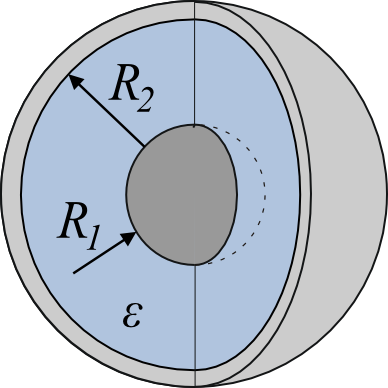
\includegraphics[scale=0.4]{Spherical_Capacitor.png} 
	\end{center}
	\vspace{-10pt}
\end{wrapfigure}

In der von uns bearbeiteten Aufgabe geht es um die Berechnung der Kapazitäten von mehreren Kugelkondensatoren.


Ein Kugelkondensator besteht aus zwei konzentrisch angeordneten Kugeln, die durch ein Isoliermaterial, genannt \emph{Dielektrikum}, getrennt werden. Die Kapazität des resultierenden Kondensators hängt von dem Verhältnis der Radien der beiden Kugeln und dem verwendeten Dielektrikum ab.

Dazu wird eine Liste von Radien --- jeweils für den Radius der inneren und der äußeren Kugel --- in Form einer Textdatei eingegeben. Zu dieser werden dann in einem Assemblerprogramm die jeweiligen Kapazitäten für verschiedene Dielektrika berechnet (in unserem Fall Hartgummi und Hartpapier).
Die Abmessungen bestehen jeweils aus zwei Radien, dem der inneren Kugel $r_{1}$ und dem der äußeren Kugel $r_{2}$.

Die Formel zur Berechnung der Kapazität eines Kugelkondensators lautet:

\begin{center} \begin{LARGE}
$ C= 4 \pi \varepsilon_{0} \varepsilon_{r} \frac{r_{1} \cdot r_{2}} {r_{2} - r_{1}} $
\end{LARGE} \end{center}
$ \varepsilon_{0} $ bezeichnet dabei die elektrische Feldkonstante und beträgt $8,85418781762 \cdot 10^{-12}$.\\
$ \varepsilon_{r} $ bezeichnet den Dielektrizitätswert des Materials (für Hartgummi $3,0$, für Hartpapier $5,0$).

\subsection{Implementierungsumgebung}
Wir verwenden zur Entwicklung das \board, ein ARM Cortex-A8-System (aufbauend auf der ARMv7-Architektur, getaktet mit 1 GHz) mit NEON-VFP. Die NEON-Architektur erlaubt es, Berechnungen mit bis zu vier Fließkommazahlen (32 bit) gleichzeitig durchzuführen, wodurch eine hohe Performanz beim \emph{Number Crunching} erreicht wird. Dieses Verfahren wird \emph{SIMD} (von ARM selbst \emph{Advanced}-SIMD) genannt.\\
Beispiele für fließkommaintensive Berechnungen sind Audioverarbeitung, 3D-Visuali-sierungen oder Physik-Simulationen.\\
Weiterhin bietet das \board 512-MB LPDDR RAM, einen High-speed USB 2.0 OTG-Port, 10/100 Ethernet, DVI-D und S-Video-Anschlüsse, Stereo-Audio out/in, einen High-capacity microSD Slot, JTAG und einen Kamera-Port, was enorme Vielfalt in den Erweiterungs- und Anwendungsmöglichkeiten bietet.
\\ \\
Unsere Entwicklungsumgebung besteht aus dem \emph{ARM Development Studio 5 für Eclipse}, \emph{GNU make} und \emph{gcc 4.7}.

\emph{DS-5} ist eine auf der Entwicklungsplattform Eclipse aufgebaute Umgebung, die eine einfach zu benutzende graphische Oberfläche zum Entwickeln, Ausführen und Debuggen von Programmen für ARM-Systeme bereitstellt. Die Einrichtung ist jedoch etwas umständlich, da DS-5 nicht ganz fehlerfrei ist und keinen klaren Leitfaden zum Erstellen eines Projekts bietet. Das Programm selbst ist kostenpflichtig, sowie nur unter einer eingeschränkten Lizenz distributiert, was eigene Erweiterungen erschwert.

\emph{GCC} ist eine der weitverbreitesten Compilersuiten, ist vollständig Open-Source und in der Lage, für alle bekannten Architekturen und Betriebssysteme C, C++ und Assemblercode zu Binärcode umzubauen, wobei zusätzlich auch umfangreiche und effektive Optimierungsoptionen vorhanden sind.

\section{Lösungsalternativen}
\subsection{Vector Floating Point (VFP)}
\subsubsection*{Vorstellung}
In der von uns enwickelten Lösung verwenden wir die Vector Floating Point Erweiterung des ARM-Prozessors. 
Diese erlaubt es uns mit \emph{single} (32 bit)- und \emph{double} (64 bit)-precision Fließkommazahlen nach dem IEEE 754-Standard zu rechnen.
\subsubsection*{Vorteile}
\begin{itemize}
\item beliebige Menge an zu verarbeitenden Daten
\item lauffähig auch auf Architekturen ohne NEON
\end{itemize}
\subsubsection*{Nachteile}
\begin{itemize}
\item eventuell langsamer, da der VFP-Koprozessor (bzw. der NEON-Befehlssatz) nicht voll genutzt wird (d.h. ohne SIMD) bzw. mehr Taktzyklen für die Berechnung benötigt werden (je nachdem, ob der schnellere \emph{VFPv3}- oder nur der \emph{VFPLite}-Koprozessor vorhanden ist)
\item VFP-Koprozessor wird benötigt
\end{itemize}
\subsection{SIMD (NEON-Coprozessor)}
\subsubsection*{Vorstellung}
In dieser alternativen Lösung wird der NEON Coprozessor von ARM verwendet, um von \emph{SIMD} (Single Instruction, Multiple Data)
zu profitieren. Das bedeutet, dass pro Instruktion nicht mit einer, sondern mit bis zu vier Zahlen gleichzeitig gerechnet werden kann. Unsere Tests haben gezeigt, dass die Berechnung dadurch mindestens um den Faktor 6 beschleunigt wird.
\subsubsection*{Vorteile}
\begin{itemize}
\item Um Faktor 6-8 schneller als VFP ohne SIMD
\end{itemize}
\subsubsection*{Nachteile}
\begin{itemize}
\item SIMD Befehle müssen jeweils zwei oder vier Fließkommazahlen verarbeiten. Falls die Eingabedatenmenge kein Vielfaches von vier ist, kann für den entsprechenden Rest nicht derselbe Code verwendet werden.
\item Der NEON Befehlssatz verfügt über keinen Divisionsbefehl. Die einzige Möglichkeit ist die Approximation des Kehrbruchs mit \emph{VRECPE} und anschließende Multiplikation.
Die einmalige Annäherung ist nicht sehr genau, durch mehrmalige Iteration des Newton-Raphson-Verfahrens mittels \emph{VRECPS} erhält man jedoch ähnliche Genauigkeit wie mit nicht-SIMD-Operationen.
\end{itemize}
\subsection{Entscheidungsprozess}
Um keine Entscheidung zugunsten einer Lösung treffen zu müssen, haben wir einfach alle Alternativen selbst implementiert, wobei bei der NEON-Variante nur der Berechnungsteil in Assembler umgesetzt wurde, die Schleifenstruktur zur Übergabe der Daten wurde dagegen in C geschrieben.
\section{Dokumentation der Implementierung}
\subsection{Entwickler-Dokumentation}
\subsubsection{Rahmenprogramm}
Das in C geschriebene Rahmenprogramm liest die Datensätze mit den Radien der Kugelkondensatoren aus einer Textdatei in den Speicher.
Mit diesen Daten werden dann drei verschiedene Implementierungsvarianten ausgeführt (Assembler mit VFP, Assembler mit NEON und Vektorisierung und die C-Referenzimplementierung), deren Ergebnisse ausgegeben werden und die dafür benötigte Zeit (in Mikrosekunden) gemessen wird.
\\\\
Zunächst werden über die Methode \emph{$datei\_lesen$} die in der Datei \emph{$ui.txt$} stehenden Datensätze eingelesen. Die einzulesende Datei muss dabei folgenden Richtlinien folgen:
\begin{verse}
$ $ Zeile 1: $\; n-1 $ \\
$ $ Zeile 2: $\; [x_{0}]_{r_{1}} \: $mm$ \: [x_{0}]_{r_{2}} \: $mm$ $ \\
$ $ $\vdots $\\
$ $ Zeile n: $\; [x_{n-1}]_{r_{1}} \: $mm$ \: [x_{n-1}]_{r_{2}}\: $mm$ $
\end{verse}
Hierbei ist $x$ (mit der Mächtigkeit $\vert x \vert = n$) die Menge aus den zu berechnenden Datensätzen bestehend aus den 2-Tupeln $(r_{1},r_{2})\in \mathbb{R}^{2} $, wobei $r_{1}$ den Radius der inneren Kugel und $r_{2}$ den Radius der äußeren Kugel bezeichnet.
\\\\
Die Methode wird mit den benötigten Parametern aufgerufen und der Rückgabewert gesichert. Dieser spezifiziert einen eventuell aufgetretenen Fehler ($\neq 0$ bei einem Fehler). Wenn ein Fehler aufgetreten ist wird dies anschließend erkannt und das Programm mit diesem Fehlerwert beendet.

Die Parameter von \emph{$datei\_lesen$} lauten wie folgt:
\begin{enumerate}
\item Name der einzulesenden Datei
\item Pointer auf ein \emph{float}-Array, in dem die inneren Radien gespeichert werden
\item Pointer auf ein \emph{float}-Array, in dem die äußeren Radien gespeichert werden
\item Pointer auf einen \emph{int}, hier wird die Länge des Datensatzes gespeichert
\end{enumerate}

\begin{lstlisting}
int erfolg = datei_lesen("ui.txt", &rad1, &rad2, &length);
if(erfolg != 0) {
	return erfolg;
}
\end{lstlisting}
Im folgenden wird auf die Arbeitsweise dieser Methode anhand von weiteren Auszügen aus dem Quelltext eingegangen.\\\\

\begin{lstlisting}[language=C]
FILE* handle = NULL;
\end{lstlisting}
Erzeugt eine Variable namens \emph{$handle$}, in der ein Pointer auf ein \emph{$FILE$}-Struct, definiert in der Headerdatei \emph{$stdio.h$} (Teil der Standard-C-Bibliotheken) gespeichert werden kann. Damit wird ein späterer Zugriff auf die einzulesende Datei ermöglicht. Zunächst wird die Variable aber auf \emph{$NULL$} gesetzt, weil noch keine Datei geöffnet wurde.


\begin{lstlisting}[language=C]
char line[MAX_LINE_LENGTH];
\end{lstlisting}
Erzeugt eine Variable namens \emph{$line$}, in der ein Array der Größe \emph{MAX\_LINE\_LENGTH} (als \emph{1024} definiert) mit Elementen vom Typ \emph{$char$} gespeichert wird. Benötigt wird diese Variable zum Speichern des Inhalts der aktuellen Zeile in der einzulesenden Datei.
\\\\
\begin{lstlisting}[language=C]
handle = fopen(filename, "r");
if(!handle) {
	fprintf(stderr,"FEHLER: Datei konnte nicht geoeffnet werden!\n");
	return 1; 
}
\end{lstlisting}
Mit \emph{fopen} wird versucht die Datei, die unter dem Pfad spezifiziert vom Parameter \emph{filename} zu finden ist, im Lesemodus (deshalb das \emph{"r"} als zweiter Parameter) zu öffnen und anschließend eine Zugriffsreferenz für die spätere Verwendung unter der vorher definierten Variable \emph{handle} zu sichern. Schlägt dies fehl, d.h. \emph{handle} hat den Wert \emph{0}, wird eine entsprechende Ausgabe an den systemweiten Error-Stream gesendet und die Methode mit dem Rückgabewert \emph{1} abgebrochen.
\\\\
\begin{lstlisting}[language=C]
if(feof(handle) || fgets(line, MAX_LINE_LENGTH, handle)==NULL) {
	fprintf(stderr,"Fehler: Datei ist leer\n");
	return 1;
}
\end{lstlisting}
Hier wird überprüft, ob es sich bei der einzulesenden Datei um eine leere Datei handelt bzw. von der Datei überhaupt gelesen werden kann. Zunächst wird mittels \emph{feof} sichergestellt, dass das Ende des Dateistreams noch nicht erreicht ist, um anschließend zu überprüfen ob die erste Zeile gelesen werden kann. Die Methode \emph{fgets} erwartet hierbei einen Pointer auf ein \emph{char}-Array (\emph{line}), in das bei einem erfolgreichen Lesevorgang die nächsten \emph{1024} (\emph{MAX\_LINE\_LENGTH}) Zeichen des Streams \emph{handle} geschrieben werden. Schlägt einer der Tests fehl, wird wiederum eine entsprechende Ausgabe an den systemweiten Error-Stream gesendet und die Methode mit dem Rückgabewert \emph{1} abgebrochen.
\\\\
\begin{lstlisting}[language=C]
*length = atoi(line);
if(*length <= 0) {
	fprintf(stderr, "Fehler: '%s' ist keine sinnvolle Zeilennummer\n", line);
	return 1;
}
\end{lstlisting}
Um die Größe des Datensatzes herauszufinden, wird hier der Inhalt der ersten Zeile mittels \emph{atoi} in einen \emph{Integer} umgewandelt, der dann im vom Parameter \emph{length} referenzierten Speicher gesichert wird. Um fehlerhafte Daten auszuschließen, wird danach überprüft, ob es sich eine sinnvolle Länge handelt ($>0$). Ist dies nicht der Fall wird eine entsprechende Fehlermeldung ausgegeben und die Methode mit dem Rückgabewert \emph{1} abgebrochen.
\\\\
\begin{lstlisting}[language=C]
*rad1 = (float*)malloc(*length * sizeof(float));
*rad2 = (float*)malloc(*length * sizeof(float));
if(!rad1 || !rad2) {
	fprintf(stderr,"Fehler: keinen Speicher bekommen\n");
	return 1;
}
\end{lstlisting}
Zunächst wird für die inneren (\emph{rad1}) und äußeren (\emph{rad2}) Radien der Kugelkondensatoren des Datensatzes versucht, entsprechend großen Speicher zu allozieren (Länge des Datensatzes multipliziert mit der Größe der Daten selbst, die ja aus \emph{float}s bestehen). Anschließend wird überprüft, ob dieser Vorgang erfolgreich ausgeführt werden konnte, wobei bei einem Fehler ähnliches passiert wie in den vorangehenden Absätzen.
\\\\
Die nachfolgende Schleife versucht, die Datei zeilenweise einzulesen und die dabei gewonnenen Daten im passenden Speicherbereich zu sichern. Dabei wird jeweils ähnlich wie zu Beginn der Methode sichergestellt, dass weder das Ende der Datei erreicht noch eine leere Zeile eingelesen wurde.
\\\\
\begin{lstlisting}[language=C]
if(sscanf(line, "%f mm %f mm", (*rad1+index), (*rad2+index)) != 2) {
	fprintf(stderr, "Fehler in Z. %d: %s\n", index, line);
	fprintf(stderr, "Ich bin mal weg\n");
	return 1;
}
\end{lstlisting}
Die Daten in der aktuellen Zeile der Datei werden hier mittels \emph{sscanf} extrahiert und an der entsprechenden Position in den Arrays gespeichert. Die Parameter dieser Funktion verhalten sich dabei gleich wie \emph{sprintf}, nur die Funktionsweise ist umgekehrt (Werte werden eingelesen statt ausgegeben). Der Rückgabewert entspricht dabei den erfolgreich ausgelesenen Werten, wenn dieser also nicht \emph{2} ist, was bedeuten würde, dass die aktuelle Zeile ein ungültiges Format hat, wird das Einlesen abgebrochen und eine entsprechende Fehlermeldung ausgegeben. Außerdem werden Gegenmaßnahmen durchgeführt, falls in der Datei zu viele (> \emph{length}: restliche Daten werden ignoriert) oder zu wenige (< \emph{length}: \emph{length} wird entsprechend geändert) Daten zu finden sind.
\\\\
Nun sollte sichergestellt sein, dass gültige Daten eingelesen wurden, diese werden dann, nachdem genügend großer Speicher für die Ergebnisse alloziert wurde der Assemblerroutine übergeben. Vorher wird noch der aktuelle Timestamp gespeichert, damit eine Zeitmessung erfolgen kann. Nachdem die Berechnung erfolgt ist, werden Auszüge aus den Ergebnissen ausgegeben sowie die benötigte Zeit.
\\\\
Abschließend wird die geöffnete Datei noch mittels \emph{fclose} geschlossen und ein Fehler ausgegeben, falls sie nicht geschlossen werden konnte.
\begin{lstlisting}[language=C]
if(fclose(handle) != 0) {
	fprintf(stderr, "Fehler: Konnte Eingabedatei nicht schließen.\n");
}
\end{lstlisting}

\subsubsection{Assemblerroutine - VFP-Version}
Der Einstiegspunkt der Assemblerroutine ist die Funktion \emph{\_calc}. Sie erwartet folgende Parameter:
\begin{enumerate}
\item 2 \emph{float}-Arrays (\emph{data1}/\emph{data2}), in denen die Abmessungen der Kondensatoren erwartet werden
\item 2 \emph{float}-Arrays (\emph{result1}/\emph{result2}), in denen die berechneten Kapazitäten für die beiden Dielektrika gespeichert werden
\item Ein \emph{int} (\emph{length}), der die Größe des Datensatzes angibt
\end{enumerate}

Im folgenden wird auf die Arbeitsweise dieser Routine anhand von Auszügen aus dem Quellcode näher eingegangen.
\begin{lstlisting}[language={[x86masm]Assembler}]
_calc :
	PUSH {r4-r10,r11}
\end{lstlisting}
Hier werden zunächst alle in der Routine verwendeten Register auf dem Stack gesichert, um sie später wiederherstellen zu können.
\\
\begin{lstlisting}[language={[x86masm]Assembler}]
	ADD r11,sp, #0x1c
\end{lstlisting}
Das Register \emph{r11} wird mit einem neuen Stackpointer beschrieben, der für den benötigten Stackframe verwendet wird. Da vorher \emph{7} Words ($7 \cdot 4 = 28$ Byte groß, ausgenommen \emph{r11} selbst) auf den Stack gepusht wurden, wird der referenzierte Speicher um \emph{28} ($1c_{16}$) Bytes erhöht. 
\\
\begin{lstlisting}[language={[x86masm]Assembler}]
	SUB sp, sp, #20
\end{lstlisting}
Vom eigentlichen Stackpointer werden nun \emph{20} Bytes (\emph{5} Words) abgezogen, da dieser Platz später zum Sichern der Parameter benötigt wird.
\\
\begin{lstlisting}[language={[x86masm]Assembler}]
	STR r0, [r11,#-0x8]
	STR r1, [r11,#-0xc]
	STR r2, [r11,#-0x10]
	STR r3, [r11,#-0x14]
	PUSH {lr}
\end{lstlisting}
Die ersten \emph{4} Parameter (\emph{r0}: data1, \emph{r1}: data2, \emph{r2}: result1, \emph{r3}: result2) werden auf dem Stack gesichert, jeder Kopiervorgang wird dabei mit einem entsprechenden Offset ausgeführt (jeweils um die Größe eines Words vermindert, beim ersten Vorgang ein Word mehr, da sonst der vorher gesicherte Wert von \emph{r11} überschrieben werden würde). Zusätzlich wird das Link-Register (\emph{lr}) auf dem Stack platziert.
\\
\begin{lstlisting}[language={[x86masm]Assembler}]
	LDR r0, [r11,#4]
	STR r0, [r11,#-0x18]
\end{lstlisting}
Der \emph{5}. Parameter (\emph{length}) wird gemäß Calling-Convention nicht direkt in einem Register übergeben, sondern befindet sich auf dem Stack. Von dort wird er zunächst in das Register \emph{r0} geladen, um ihn anschließend an der von uns benötigten Position im Stack zu sichern.
\begin{lstlisting}[language={[x86masm]Assembler}]
	LDR r1, [r11,#-0x8]
	LDR r2, [r11,#-0xc]
	LDR r3, [r11,#-0x10]
	LDR r4, [r11,#-0x14]
\end{lstlisting}
Hier werden die restlichen Parameter wieder in die benötigten Register geschrieben (\emph{r1}: data1, \emph{r2}: data2, \emph{r3}: result1, \emph{r4}: result2).
\\
\begin{lstlisting}[language={[x86masm]Assembler}]
	VLDR.F32 s0, _M_PI
	VLDR.F32 s3, _M_E_0
	VMUL.F32 s0, s0, s3
	VLDR.F32 s3, _M_4
	VMUL.F32 s3, s0, s3
\end{lstlisting}
Nun kann die eigentliche Berechnung beginnen: Der konstante Faktor der Formel ($4 \cdot \pi \cdot \varepsilon_{0}$) wird vorberechnet. Dazu werden zunächst der Wert von $\pi$ und $\varepsilon_{0}$ in den Single-Precision-Registern \emph{s0} und \emph{s3} gespeichert, damit mit diesen Werten Fließkomma-Operationen durchgeführt werden können. Anschließend werden diese beiden Zahlen multipliziert und auf ähnliche Weise mit dem Faktor $4$ verrechnet. Das Ergebnis (also der konstante Teil der Formel) steht nun im Register \emph{s3}. Ausgeführt werden all diese (und auch spätere) Befehle mit \emph{32}bit-Fließkommazahlen.
\\
\begin{lstlisting}[language={[x86masm]Assembler}]
	SUB r0, r0, #1
loop :
	ADD r5, r1, r0, LSL #2
	ADD r6, r2, r0, LSL #2
	ADD r7, r3, r0, LSL #2
	ADD r8, r4, r0, LSL #2
\end{lstlisting}
Um die richtige Anzahl an Schleifendurchläufen auszuführen, muss von der Größe des Datensatzes (Parameter \emph{length}, in \emph{r0} gespeichert) noch \emph{1} subtrahiert werden, da Arrays ja bekanntlich \emph{0}-basiert sind. Anschließend werden mit einem Label (\emph{loop}) das Beginn der Schleife markiert und die Pointer (für die Eingabe/Ausgabe) an die richtige Position gesetzt. Dafür wird die Zählvariable (\emph{r0}) zunächst mittels \emph{LSL \#2} (Logical Shift Left, entspricht Multiplikation mit $2^{n}$) über den Barrel-Shifter mit $4$ multipliziert, um gültige Speicheroffsets zu bekommen (ein \emph{float} ist \emph{4} Byte groß).
\\
\begin{lstlisting}[language={[x86masm]Assembler}]
	VLDR.F32 s0, [r5]
	VLDR.F32 s1, [r6]
	VLDR.F32 s2, _E_GUMMI
	BL _capacity
	VSTR.F32 s0, [r7]
\end{lstlisting}
Zunächst werden die an den vorher berechneten Speicheradressen stehenden Werte (also der innere/äußere Radius des Kugelkondensators) in die für die Routine \emph{\_capacity} (führt eigentliche Berechnung der Kapazität aus) benötigten Register kopiert und der Dielektrizitätswert für Hartgummi in das richtige Register geladen. Dann wird mittels \emph{BL} ein Sprung zu dieser Routine durchgeführt, wobei die Rücksprungadresse implizit im Link-Register gesichert wird. Ist die Routine fertig, wird das Ergebnis, dass per Konvention in Register \emph{s0} gespeichert wurde, an die richtige Stelle im Ergebnis-Array geschrieben.
Danach wird dasselbe (mit anderen Speicheradressen) noch einmal für das Dielektrikum Hartpapier durchgeführt.
\\
\begin{lstlisting}[language={[x86masm]Assembler}]
	SUBS r0, r0, #1
	BPL loop
\end{lstlisting} 
Nach dem Dekrementieren der Zählvariable (mit Operationssuffix \emph{S}, um entsprechende Flags zu aktualisieren), wird, falls die Subtraktion kein negatives Ergebnis verursacht hat (d.h. $r0 >= 0$, angezeigt über die \emph{N}-Flag) wieder an den Schleifenanfang gesprungen und die Datenverarbeitung fortgesetzt.
\\
\begin{lstlisting}[language={[x86masm]Assembler}]
	POP {lr}
	SUB sp, r11, #0x1c
	POP {r4-r10,r11}
	BX lr
\end{lstlisting}
Am Ende werden alle (vorher gesicherten) verwendeten Register wiederhergestellt, der Stackframe wiederhergestellt und ein Rücksprung zu der im Link-Register gespeicherten Adresse veranlasst.
\\\\
Im folgenden wird die Routine \emph{\_capacity}, die die eigentliche Berechnung der Kapazität durchführt, näher beschrieben. Diese Funktion erwartet als Parameter 4 \emph{float}-Werte (innerer/äußerer Radius, Dielektrizitätswert und konstanter Teil der Formel wie oben erläutert) und liefert das Ergebnis in Register \emph{s0} zurück.
\\
\begin{lstlisting}[language={[x86masm]Assembler}]
_capacity :
	PUSH {r5-r7,r11}
	ADD r11,sp, #0xc
	VPUSH {s3-s5}
\end{lstlisting}
Ähnlich wie vorangehend beschrieben werden hier die verwendeten Register auf dem Stack gesichert und ein neuer Stackframe erstellt. \emph{VPUSH} sichert hierbei auch die verwendeten VFP-Register.
\\
\begin{lstlisting}[language={[x86masm]Assembler}]
	VSUB.F32 s4, s1, s0
	VDIV.F32 s4, s0, s4
	VMUL.F32 s4, s4, s1
	VMUL.F32 s0, s3, s2
	VMUL.F32 s0, s0, s4
\end{lstlisting}
Dieser Teil führt die Berechnung der Kapazität aus: Zunächst wird der innere Radius vom äußeren subtrahiert, anschließend wird mit dem Produkt aus den Radien der Quotient gebildet. Am Schluss wird das noch mit dem konstanten Teil der Formel und dem Dielektrizitätswert multipliziert, das Ergebnis liegt nun im Register \emph{s0}.
\\
\begin{lstlisting}[language={[x86masm]Assembler}]
	VPOP {s3-s5}
	SUB sp, r11, #0xc
	POP {r5-r7,r11}
	BX lr
\end{lstlisting}
Nun werden die verwendeten (und vorher gesicherten) Register wiederhergestellt, der Stackframe zurückgesetzt und mittels \emph{BX} ein Rücksprung zum Aufrufer (bzw. an die im Link-Register gespeicherte Adresse) veranlasst.

\subsubsection{Assemblerroutine - NEON-Version}

Da wir uns zunächst für eine Implementierung ohne SIMD-Vektorisierung entschieden haben, haben wir den Assembler-Aufrufcode nicht an die Vektorisierung angepasst und haben die NEON-Alternative direkt mittels C-Code angesprochen. Der C-Code, der zum Aufruf der Funktion benötigt wird, wird hier nicht näher erläutert, da er zum Verständnis keinerlei Erklärung bedarf.

Die Routine \emph{\_fast\_capacity} berechnet für 4 Kugelkondensatoren die Kapazität mit jeweils 2 Dielektrika. Sie erwartet --- wie \emph{\_calc} --- als Parameter 2 \emph{float}-Arrays mit Mindestgröße 4, hieraus werden die Radien der Kondensatoren gelesen; ein \emph{2} Elemente großes \emph{float}-Array, in dem die Dielektrizitätswerte stehen und \emph{2} \emph{float}-Arrays, in denen die Ergebnisse gespeichert werden.
\\
\begin{lstlisting}[language={[x86masm]Assembler}]
_fast_capacity :
	PUSH {r11}
	ADD r11,sp,#0x0
	VPUSH {q0-q5}
	VLDM r2, {d0}
	VLDM r0, {q1}
	VLDM r1, {q2}
\end{lstlisting}
Zu Beginn werden sämtliche verwendeten Register sowie der Stackpointer gesichert und die übergebenen Parameter in die NEON-Register geladen. \emph{VLDM} lädt dabei mehrere Werte in ein entsprechendes Vektorregister (\emph{Q}uad-Register: \emph{4} Werte, \emph{D}ouble-Register: \emph{2} Werte). Die inneren/äußeren Radien befinden sich nun also in den Registern \emph{q1}/\emph{q2}, die beiden Dielektrizitätswerte im Register \emph{d0}.
\\
\begin{lstlisting}[language={[x86masm]Assembler}]
	VSUB.F32 q4, q2, q1
	VRECPE.F32 q3, q4
\end{lstlisting}
Danach wird mit der eigentlichen Berechnung begonnen, die im folgenden immer mit 4 Werten gleichzeitig operiert. Zunächst wird die Differenz aus den inneren und äußeren Radien gebildet, um dieses Ergebnis anschließend im ersten Schritt der Kehrbruchapproximation zu verwenden, da NEON direkte Division nicht unterstützt. \emph{VRECPE} führt dabei eine bisweilen etwas ungenaue Approximation von $\frac{1}{d}$ (in unserem Fall also $\frac{1}{r2-r1}$) aus, die danach noch weiter präzisiert wird.
\\
\begin{lstlisting}[language={[x86masm]Assembler}]
	VRECPS.F32 q5, q3, q4
	VMUL.F32 q3, q5, q3
	VRECPS.F32 q5, q3, q4
	VMUL.F32 q3, q5, q3
\end{lstlisting}
Um diesen Kehrbruch ($\frac{1}{d}$) genauer anzunähern, werden hier 2 Schritte der Newton-Raphson-Iteration ($x_{n+1}=x_{n} \cdot (2 - x_{n} \cdot d)$) durchgeführt (als Startwert wird die vorher berechnete Approximation in Register \emph{q3} verwendet), die im NEON-Befehlssatz schon fest eingebaut ist. \emph{VRECPS} errechnet den zweiten Faktor der Formel ($2 - x_{n} \cdot d$), anschließend muss noch mit $x_{n}$ multipliziert werden. Unsere Tests haben ergeben, dass eine zweimalige Durchführung dieser Iteration genügende Genauigkeit ($\approx$ 7 signifikante Stellen) liefert.
\\
\begin{lstlisting}[language={[x86masm]Assembler}]
	VMUL.F32 q3, q3, q1
	VMUL.F32 q3, q3, q2
	VLDR d1, _M_4_PI
	VMUL.F32 q3, q3, d1[0]
	VMUL.F32 q3, q3, d1[1]
	VLDR d1, _M_E_0
	VMUL.F32 q3, q3, d1[0]
\end{lstlisting}
Nach Multiplikation der bisherigen Ergebnisse mit $r1 \cdot r2$ werden anschließend $\pi$ und $4$ in das Register \emph{d1} geladen, um die Zwischenergebnisse mit diesen Skalaren zu multiplizieren. Dasselbe wird mit dem Faktor $\varepsilon_{0}$ gemacht.
\\
\begin{lstlisting}[language={[x86masm]Assembler}]
	VMUL.F32 q4, q3, d0[0]
	VMUL.F32 q5, q3, d0[1]
\end{lstlisting}
Die endgültigen Ergebnisse erhält man letztendlich durch Multiplikation mit den beiden Dielektrizitätswerten, was hier durchgeführt wird. Anschließend befinden sich die Kapazitäten jeweils in den Registern \emph{q4} für Dielektrizitätswert \emph{1} und \emph{q5} für Dielektrizitätswert \emph{2}.
\\
\begin{lstlisting}[language={[x86masm]Assembler}]
	VSTM r3, {q4}
	LDR r0, [r11,#0x4]
	VSTM r0, {q5}
	VPOP {q0-q5}
	SUB sp,r11, #0x0
	POP {r11}
	BX lr
\end{lstlisting}
Damit der Aufrufer später auf die Ergebnisse zugreifen kann, müssen diese noch in den richtigen Speicherbereich kopiert werden. Dafür existiert der Befehl \emph{VSTM}, der (ähnlich wie bei \emph{VLDM}) mehrere Werte aus einem NEON-Register in den Speicherbereich, das von einem Standardregister referenziert wird, schreiben kann. Für \emph{result1} (in Register \emph{r3}) funktioniert das ohne Probleme, für \emph{result2}, dessen Pointer gemäß Calling-Convention auf dem Stack übergeben wurde, ist ein weiterer Schritt nötig --- die richtige Adresse muss zunächst vom Stack geholt werden. Anschließend werden die zuvor gesicherten Register und der Stackpointer wieder zurückgeschrieben und es wird mittels \emph{BX} wieder an den Aufrufer (Adresse im Link-Register) zurückgesprungen.
\subsubsection{Optimierungen}
Durch Vorberechnung des konstanten Faktors der Formel ($4 \cdot \pi \cdot \varepsilon_{0}$) kann dieser in allen späteren Berechnungen wiederverwendet werden, was einigen Aufwand erspart. Diese Optimierung wurde nur in der VFP-Variante umgesetzt, da nur hier auch eine Schleifenstruktur implementiert wurde. Bei der NEON-Alternative ist also zusätzliches Optimierungspotential gegeben.\\
Die effiziente (minimale) Verwendung der verfügbaren Register bietet weiterhin Optimierungsmöglichkeiten. Hier haben wir versucht, den idealen Kompromiss zwischen Effizienz und Lesbarkeit zu finden.\\
\subsection{Benutzer-Dokumentation}
In dem Ordner in dem die kompilierte Binary liegt, muss der Benutzer eine \emph{ui.txt} anlegen. In der ersten Zeile steht die Anzahl der Zeilen der Datei minus eins. In den folgenden Zeilen stehen die inneren und äußeren Radien der Kugenkondensatoren, deren Kapazitäten berechnet werden sollen. Die folgenden Zeilen sind im Format \emph{Radius1 mm Radius2 mm} .

Um die Kapazitäten zu berechnen muss der Benuter einfach die Binary ohne weitere Parameter in der Konsole ausführen. Die Ausgabe zeigt nur 4 Ergebnisse: Das erste, die an den Stellen 
$n * \frac{1}{3}$ und
$n * \frac{2}{3}$
und das letzte Ergebnis. Wobei \emph{n} die Anzahl der Werte ist.
\section{Ergebnisse}
\subsection{Vergleich von Assembler und C-Code}
\subsubsection{Genauigkeit der Ergebnisse}
Die Ergebnisse des Assemblercodes weichen um maximal 0,000135 Promille von den Ergebnissen des C-Codes ab. Das heißt die Ergebnisse sind auf 5 Stellen nach dem Komma genau.

Die  Ergebnisse des Assemblercodes mit NEON-Befehlssatz weichen um maximal 0,000225 Promille von den Ergebnissen des C-Codes ab. Die Ergebnisse sind wieder auf 5 Stellen nach dem Komma genau.
\subsubsection{Laufzeit}
Für die Berechnung der Kapazitäten von 100000 Wertepaaren benötigt der C-Code im Durchschnitt ca. 25600 µs, der Assemblercode ca. 12800 µs und der Assemblercode mit NEON-Befehlssatz nur ca. 3900µs.Damit ist der Assemblercode ca. 50\% schneller und mit NEON sogar ca. 84\% schneller als der C-Code.
\subsection{Analyse und Bewertung}
%%TODO
\end{document}


